In this chapter, evaluation for Kernel-based NFCI is described. 
\subsection{Evaluation environment}
Evaluation environment consists of hypervisor and three VMs on top of it. On one of the VM runs Kernel-based NFCI and on the others runs generic kernel. Table \ref{tbl: spec1} and \ref{tbl: spec2} shows the machine specifications of hypervisor and VM respectively. Two experiments will be conducted in this environment.  

\begin{table}
	\centering
	\begin{tabular}{|c||c|}
		\hline
		OS & Ubuntu16.04 (x86\_64) \\
		\hline
		CPU & Intel-Xeon (X5690) 3.47GHz (24 cores with HT) \\
		\hline
		Memory & 48GB \\
		\hline
		VMM & KVM \\
		\hline
	\end{tabular}
	\caption{Machine Specification of hypervisor}
	\label{tbl: spec1}
\end{table}

\begin{table}
	\centering
	\begin{tabular}{|c||c|}
		\hline
		OS &  \shortstack{Ubuntu16.04 (x86\_64) / \\ Linux 4.4.90 with Kernel-based NFCI} \tabularnewline
		\hline
		vCPU & 4 cores \tabularnewline
		\hline
		Memory & 8GB \tabularnewline
		\hline
		vNIC & virtio-net \tabularnewline
		\hline
	\end{tabular}
	\caption{Machine Specification of Virtual Machines} 
	\label{tbl: spec2}
\end{table}

\begin{figure*}
	\centering
	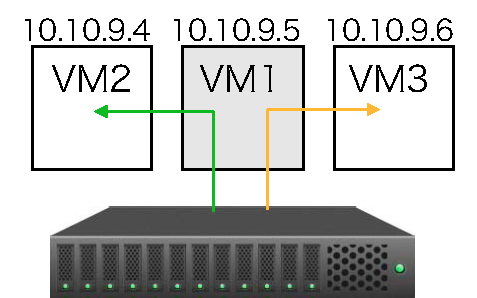
\includegraphics[width=65mm]{pics/env1.pdf}
	\caption{Direction of flows in experiment1}
	\label{fig: exp1}
\end{figure*}

\begin{figure*}
	\centering
	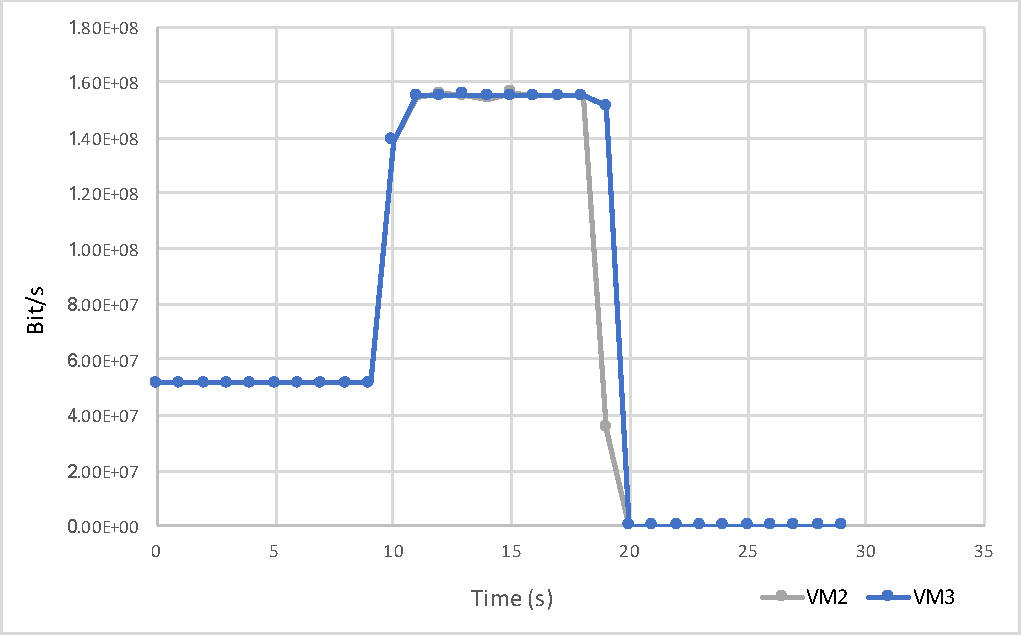
\includegraphics[width=120mm]{pics/throughput.pdf}
	\caption{Throughput at VM2 and VM3}
	\label{fig: result1}
\end{figure*}

\subsection{NF chaining performance}
To evaluate the performance of NF chaining, the following Experiment 1 is conducted. On VM1, Kernel-based NFCI executes chaining of two NFs, DoS Attack Denial (DAD) and DNAT. 

DAD counts the number of packets per flow. If in the previous 10 seconds the counter exceeds the threshold, all the packet in the flow will be dropped for the next 10 seconds. For this experiment the threshold of any flow is set to be 100Mbps. 

The chaining proceeds as follows: Hypervisor sends out two UDP flows to VM1 (10.10.9.5), flow1 having destination port number 53 (DNS protocol) and another flow2 having destination port number 123. The traffic is first chained with DAD and if the packet is not dropped, DNAT is processed. DNAT changes destination IP address to 10.10.9.4 (VM2) if it is flow1 and to 10.10.9.6 if it is flow2. So as shown in \ref{fig: exp1}, two flows originally destined to VM1 is split to VM2 and VM3. 

These two flows are sent for 30 seconds, first 10 seconds at rate of 50Mbps, next 10 seconds at 150Mbps and last 10 seconds at 100Mbps. 

The throughput at VM2 and VM3 is shown in the Figure \ref{fig: result1}.
Since both of the throughput has similar value, it proves that the DNAT is working properly to split two flows to VM2 and VM3. The last 10 seconds both of flows have 0Mbps throughput. This is because from 10 to 20 seconds the traffic is exceeding 100Mbps and DAD started dropping all the packet from 20s. 


\subsection{Evaluation of resource consumption}
Resource consumption when NF chaining is running to process traffic of 1Gbps $\times 2 $ is evaluated. Similar to Experiment 1, two UDP flows are sent to VM1 and split to VM2 and VM3 by DNAT. The difference is that the the two flow is transmitted at rate of 1Gbps for only 10 seconds. So the first NF "DAD" will work only as packet counting and blocking of packets will not triggered because there will be not packets in the next 10 seconds. Value of memory usage and CPU utilization is measured by vmstat command. 

When idle (no traffic processing is running), average memory usage was 766664 Kbytes. When NF chaining at rate of 1Gbps $\times 2 $ is taking place, there were only average 20Kbytes of increase. CPU utilization showed 0\% in both case of idle and processing. This indicates that NF chaining requires little amount of CPU processing. To get detailed information about used CPU time, I used dynamic tracing tool "BCC". Especially, a program that summarizes task on-CPU time as histogram is used. This shows how long tasks spent on the CPU before being descheduled. As shown in \ref{fig: cpudist}, the number of tasks that are on-CPU for 2048-4095 usecs is the highest in both cases when processing and idle. And the number of tasks when processing is roughly twice as much as when idle. In summary, it costs about twice the CPU time for processing but the overall CPU utilization still remains 0\%. 

\begin{table}
	\centering
	\begin{tabular}{|c|c|c|}
	\hline
	 & idle & processing \\
	 \hline
	 Memory Usage (KByte) & 766664 & 766844 \\
	 \hline
	 CPU Utilization (\%) & 0 & 0 \\
	 \hline
	\end{tabular}
	\caption{Comparison of resource consumption}
	\label{tbl: resource}
\end{table}

\begin{figure*}
	\centering
	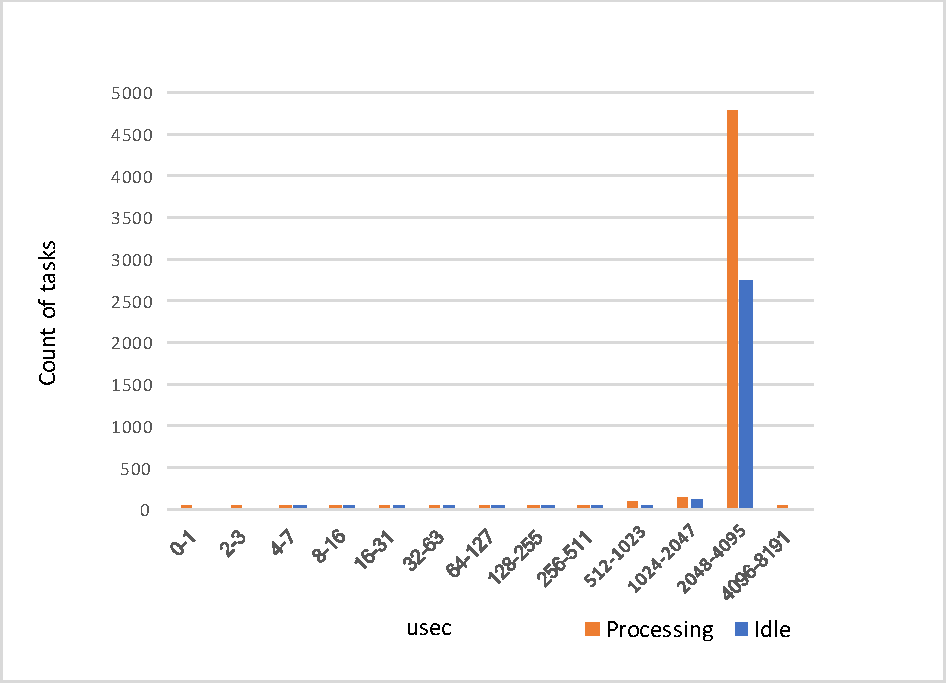
\includegraphics[width=120mm]{pics/cpudist.pdf}
	\caption{Histogram of tasks on-CPU time}
	\label{fig: cpudist}
\end{figure*}

\subsection{Evaluation of NF chaining at high traffic rate}
In addition to the evaluation of resource consumption in experiment 2, throughput is measured here. As comparison, the throughput when routing the same flows on generic OS is measured, as shown in \ref{fig: env2}. Table \ref{tbl: throughput} shows that throughput of both flows in NFC have only few kilobytes less than just routing. This proves that NFC provides equally well throughput compared with only routing at 1Gbps.

\begin{figure*}
	\centering
	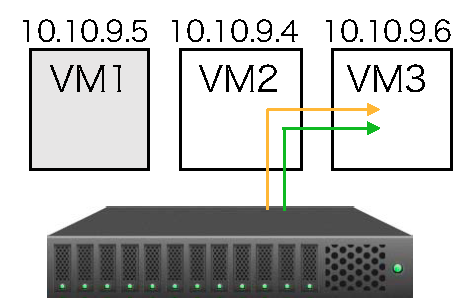
\includegraphics[width=65mm]{pics/env2.pdf}
	\caption{Routing of flows among general OSs}
	\label{fig: env2}
\end{figure*}

\begin{table}
	\centering
	\begin{tabular}{|c|c|c|}
	\hline
	 & Routing & NFC \\
	 \hline
	 flow1 (Kbps) & 801.6 & 797 \\
	 \hline
	 flow2 (Kbsp) & 804 & 800 \\
	 \hline
	\end{tabular}
	\caption{Comparison of throughput}
	\label{tbl: throughput}
\end{table}






